\chapter{Theoretical Prequisites}

\section{Microfluidics}
conservation of mass, momentum
reynolds number
\subsection{Flow Field inside Microchannels}
Navier-Stokes-Approximation for Hagen-Poiseuille
\subsection{Particles in Microfluidics}
Stokes Drag Force
Gravity
Magnetic Force
Friction
Interface-Forces
\subsection{•}

\section{Surface Chemistry}
\subsection{Carbodiimide Crosslinker Chemistry}
EDC-NHS-Activation
sulfo-NHS vs. NHS
\begin{figure}[hbtp]
\centering
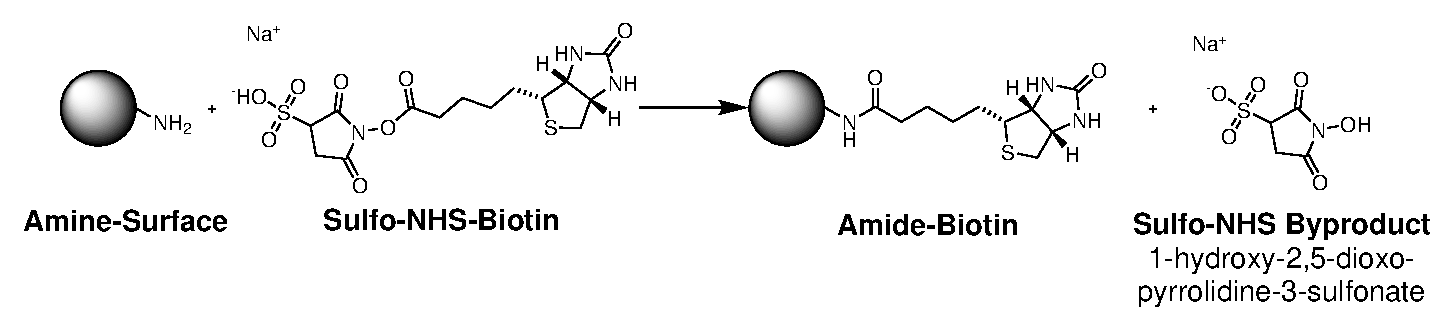
\includegraphics[width=\textwidth]{./Ressources/Chemistry/Sulfo-NHS.eps}
\caption{TestSvg}
\label{fig:Chem:NH2-NHS}
\end{figure}

\begin{figure}[hbtp]
\centering
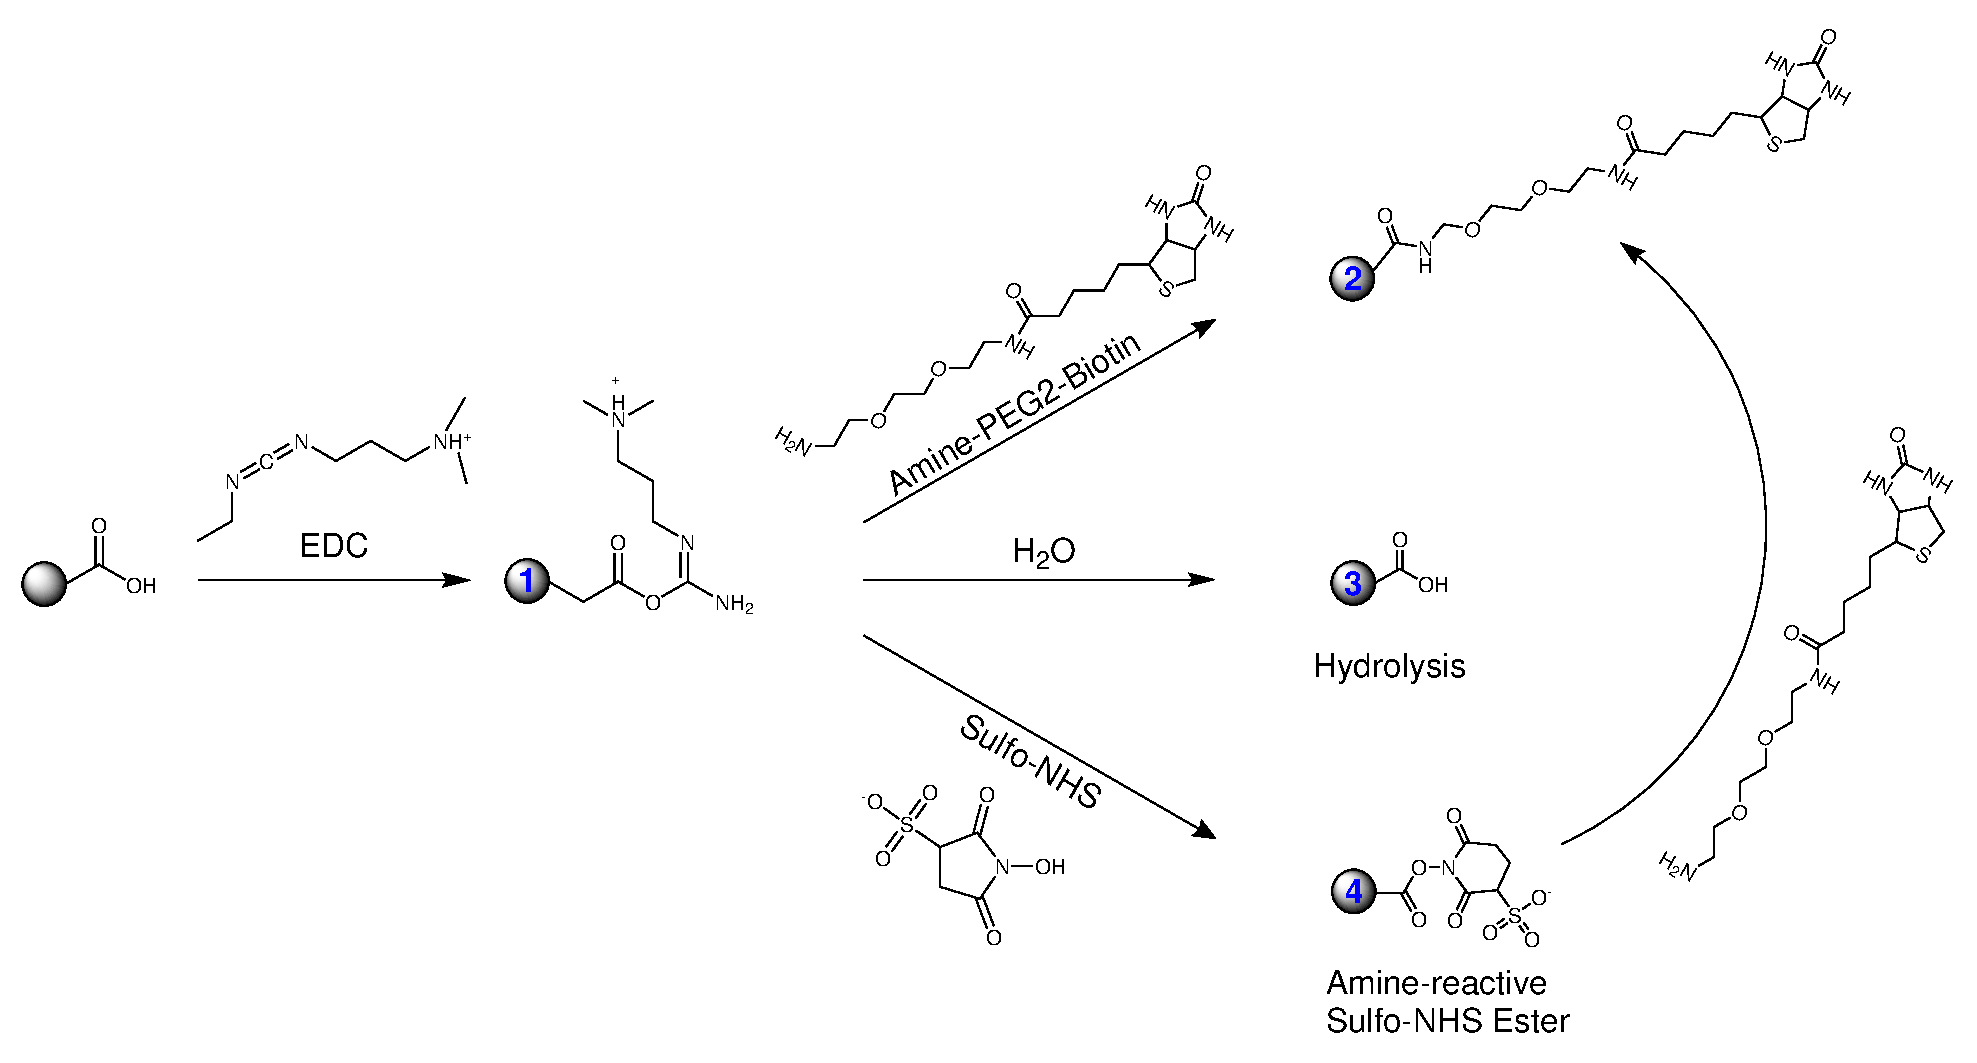
\includegraphics[width=\textwidth]{./Ressources/Chemistry/EDC-NHS.eps}
\caption{TestSvg}
\label{fig:Chem:COOH-EDC-NHS}
\end{figure}

\section{MRCyte}
Short intro over MRCyte
Foto of setup with arrows to necessary parts
Microscope
Stages
PEEK holder
Helmholtz coils
Kepco
MFLI
DAQ
\subsection{Focusing Structures}
test,test
\subsection{GMR}
Different produced GMR stacks
Wheatstone Bridge setup
Magnet alignment
\subsubsection{Hysteresis Alignment}
test,test
\subsection{Electrical Circuit}
Ground
PCB
Stacked PCBs with spacer
\subsection{Electronic Readout}
test,test
\subsubsection{Single GMR}
test,test
\subsubsection{Dual GMR}
one MFLI supplies both at same freuqency. Aux Trigger tested, but no advantage.


